\chapter{Aufbau}

\section{Übersicht des Systems}


\begin{figure}[H]
	\begin{center}
		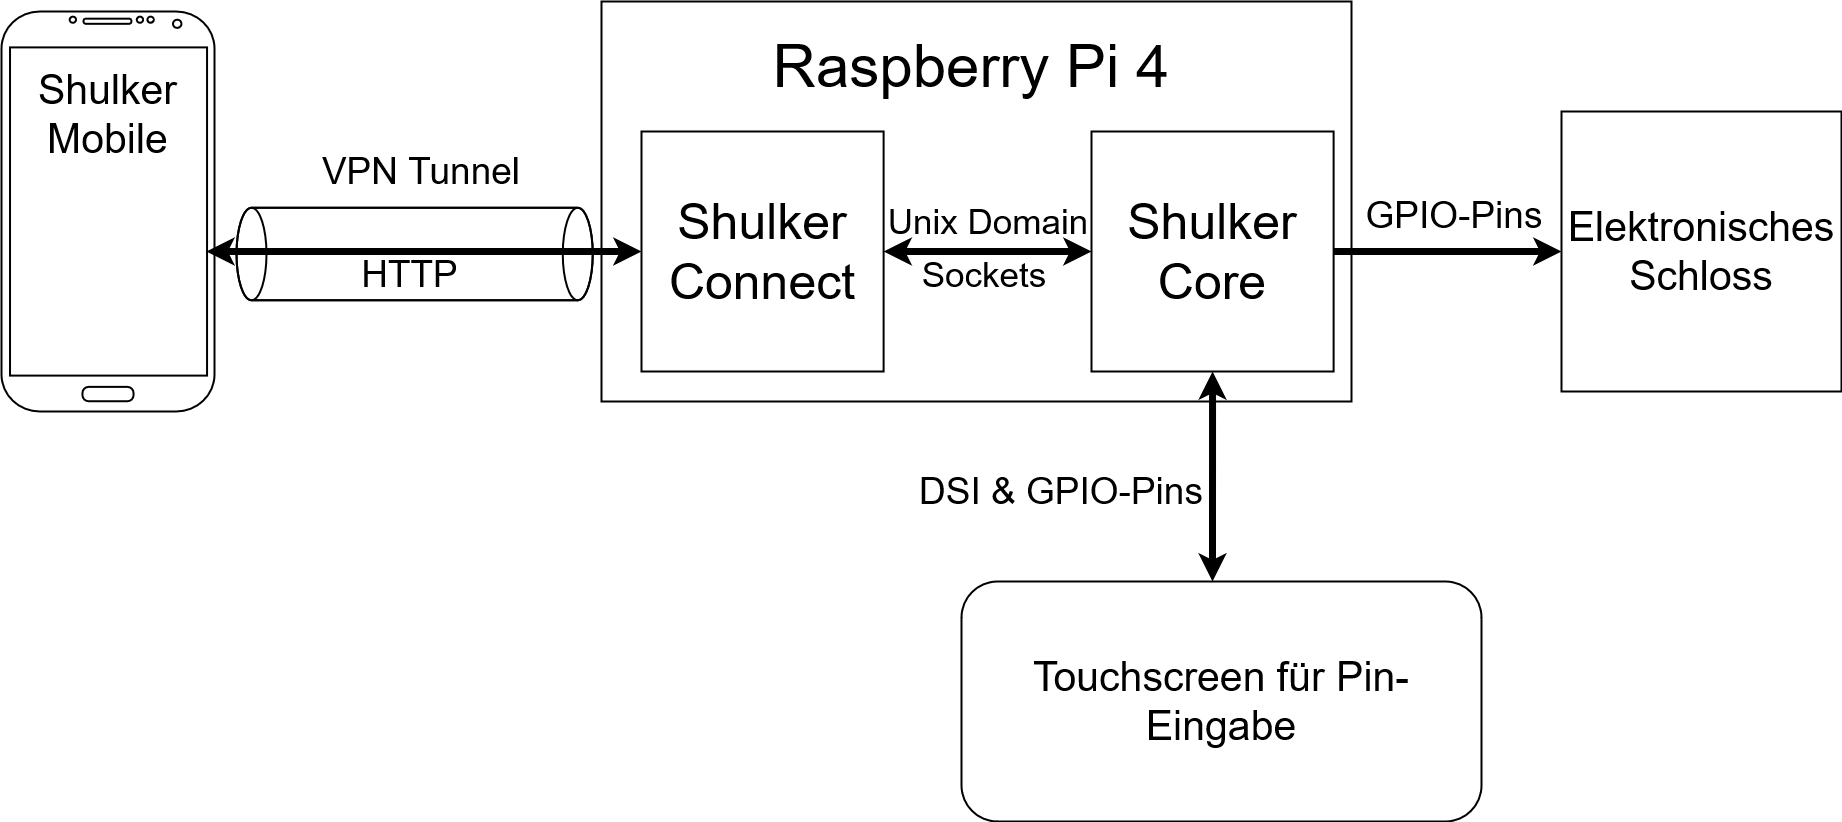
\includegraphics[width=1\textwidth]{images/Intro/Leitbild.png}
		\caption{Aufbau von \textbf{Shulker}}
	\end{center}
\end{figure}

Das Projekt setzt sich aus folgenden \textbf{drei} Komponenten zusammen:


\begin{itemize}
    \item \textbf{Shulker-Mobile}: Shulker-Mobile ist eine Smartphone-App, mit der das Türschloss verwalten werden kann.
    \item \textbf{Shulker-Connect}: Shulker-Connect ist ein auf dem Raspberry-Pi laufender Webserver, der als Schnittstelle für die Kommunikation zum Türschloss dient. Shulker-Mobile kommuniziert über einen IPsec VPN-Tunnel mit Shulker-Connect.
    \item \textbf{Shulker-Core}: Shulker-Core ist eine auf dem Raspberry-Pi laufende Software, die die Benutzeroberfläche des Touchscreens und das elektrische Schloss selbst steuert. Shulker-Core kommuniziert über Unix Domain Sockets mit Shulker-Connect.
\end{itemize}

Eine genaue Beschreibung der einzelnen Komponenten folgt in späteren Teilen der Diplomschrift. 

\section{Testumgebung}

Zu Test- und Demonstrationszwecken wurde ein Vorzeigemodell erstellt.
